\documentclass[aspectratio=169,dvipsnames]{beamer}
\usepackage[utf8]{inputenc}
\usepackage[english]{babel}
\usepackage{graphicx,hyperref,icmc,url}
\usepackage{subcaption}
\usepackage{multirow}
\usepackage{minted}
\usepackage{listings}
\usepackage{tikz}
\usepackage{array}
\usepackage{xcolor, soul}  
\usepackage{mathtools}


\usepackage{listings}% http://ctan.org/pkg/listings
\usepackage{graphbox}
\usepackage{booktabs}
\usepackage{aircraftshapes}
\newcommand{\destaq}[1]{\textcolor{BlueViolet}{\textbf{#1}}}
\newcommand\todo[1]{\colorbox{green}{#1}}

\definecolor{greenMW}{rgb}{0.0, 0.75, 0.0} % Define the greenMW color
\definecolor{orange}{rgb}{1.0, 0.65, 0.0} % Define the orange color
\definecolor{blue}{rgb}{0.0, 0.0, 1.0} % Define the blue color


% The title of the presentation:
%  - first a short version which is visible at the bottom of each slide;
%  - second the full title shown on the title slide;
\title[GraphML for Flight Delay Prediction due to Holding Manouver
]{GraphML for Flight Delay Prediction due to Holding Manouver
}

% Optional: a subtitle to be displayed on the title slide


% The author(s) of the presentation:
%  - again first a short version to be displayed at the bottom;
%  - next the full list of authors, which may include contact information;
\author[Jorge Luiz Franco]{Jorge Luiz Franco\\ \bigskip
\textsc{Undergraduate Program in Computer Science}\\ \bigskip
Advisor: Prof. Filipe Alves Neto Verri, Ph.D.}

% \\ \bigskip
    % \large{}

% The institute:
%  - to start the name of the university as displayed on the top of each slide
%    this can be adjusted such that you can also create a Dutch version
%  - next the institute information as displayed on the title slide
\institute[ICMC/USP]{Universidade de São Paulo - ICMC}

% Add a date and possibly the name of the event to the slides
%  - again first a short version to be shown at the bottom of each slide
%  - second the full date and event name for the title slide
\date[2024]{\footnotesize{June 17, 2024}}

\sloppy

\AtBeginSection[]
{
    \begin{frame}<beamer>{Summary}
        \tableofcontents[currentsection]
    \end{frame}
}

\begin{document}
    
    \begin{frame}[plain]
        \titlepage
    \end{frame}
    
    \begin{frame}
      \frametitle{Summary}
      \tableofcontents
    \end{frame}
    
%%%%%%%%%%%%%%%%%%%%%%%%%%%%%%%%%%%%%%%%%%%%%%%%%%%%%%%%%%%%%%%%

% Introduction
% Materials and Methods
%   Datasets
%   MST
%   OPF
% Experiments
%   Initial
%   DTW
%   Pruning and Improvements
%   Batch-Tests
%   Results
%   Difficulties, limitations, and future works

\section{Introduction}

\begin{frame}{Motivation}
\begin{itemize}
    \item Growing importance of efficient last-mile delivery logistics.
    \item Use of drones (Unmanned Aerial Vehicles, UAVs) for overcoming traffic constraints, reducing delivery times, and lowering operational costs.
    \item Significant increase in literature on Delivery Drones in recent years \cite{DUKKANCI2023}.
\end{itemize}
\end{frame}

\begin{frame}{Introduction to Last-Mile Delivery Drones}
    \begin{figure}
      \begin{columns}
        \column{.3\linewidth}
        \caption{Drones Congestion in a high-traffic Last Mile Delivery context. \\ Source: \cite{imageDronesCongestion}}
        \label{fig:example left}
        \column{.65\linewidth}
        \includegraphics[width=\textwidth]{img/Drone Congestion.jpg}
      \end{columns}
    \end{figure}

\end{frame}

\begin{frame}{Introduction to Last-Mile Delivery Drones}
\destaq{Last Mile Delivery Drones (LMDD)}
\begin{itemize}
    \item Heterogeneous research area:
    \begin{itemize}
        \item Combining drones and trucks.
        \item Linear integer modeling.
        \item Fuzzy logic for uncertainties.
        \item Multi-objective optimization.
        \item Exclusive drone-based solutions.
    \end{itemize}
    \item \textbf{Complex Systems Decentralized Approach}:
    \begin{itemize}
        \item Tradable permit model for multi-agent airspace use \cite{Verri}.
    \end{itemize}
\end{itemize}

\end{frame}

\begin{frame}{Related Work and Centralized Control}
\begin{itemize}
    \item \textbf{Necessity of Air Traffic Management}:
    \begin{itemize}
        \item Most centralized models don't address collision avoidance \cite{DUKKANCI2023}.
        \item Ensuring optimal path planning and efficient airspace control.
    \end{itemize}
    \item \textbf{Centralized Control and UTM}:
    \begin{itemize}
        \item \textbf{Centralized Control}:
        \begin{itemize}
            \item Federal Aviation Administration (FAA) and NASA's Unmanned Aircraft System Traffic Management (UTM) \cite{nasa}.
            \item Ensures organized, legislative-backed airspace control.
        \end{itemize}
        \item \textbf{Decentralized Models}:
        \begin{itemize}
            \item Novel but complex in scalability and regulatory compliance.
        \end{itemize}
    \end{itemize}
\end{itemize}
\end{frame}


\begin{frame}{Proposed Approach}
\begin{itemize}
    \item \textbf{Aispace Control and MAPF Approach}:
    \begin{itemize}
        \item Multi-Agent Path Finding (MAPF) is a solution for addressing spatial characteristics and collision avoidance.
    \end{itemize}
    \item \textbf{Proposed Strategy}:
    \begin{itemize}
        \item Employing MAPF strategy for Last Mile Delivery Drone problem.
        \item Three approaches: MILP, heuristic and hybrid.
        \item Use of prioritized planning \cite{7138650} and conflict-based search \cite{SHARON201540} to manage computational complexity in the heuristic.
        \item Comparing the MILP with the heuristic.
        \item Qualitative comparison between centralized and decentralized approaches.
    \end{itemize}
\end{itemize}
\end{frame}




\section{Problem Description}

\begin{frame}{LMDD as MAPF}
    \begin{itemize}
        \item Tasks for each agent (drone) described by tuples:
        \[
        task_i \coloneq \{(x_{\text{start}_i}, y_{\text{start}_i}) , (x_{\text{goal}_i}, y_{\text{goal}_i})\}, \forall \text{ drone } d_i
        \]
        \item Grid bounds: $x \leq X, y \leq Y$.
        \item Goal: find paths $P_{d_i}$ making the path length as short as possible.
    \end{itemize}
\end{frame}

\begin{frame}{Path Planning and Constraints}
    \begin{itemize}
        \item Drones limited to four principal movements: upward $(x, y+1)$, downward $(x, y-1)$, rightward $(x+1, y)$, and leftward $(x-1, y)$.
        \item Adjacency: $(x_1,y_1)$ is adjacent to $(x_2,y_2)$ $\iff |x_2-x_1| + |y_2-y_1| = 1$.
        \item New decision variable: $t_{\text{begin}}$ (arrival time).
    \end{itemize}
\end{frame}

\begin{frame}{LMDD Goals}
    \begin{itemize}
        \item Given time $T$, minimize the sum of distances of all drones.
        \item Allow drones to wait in cells and choose entry time.
        \item Non-weighted distances make the problem easier than standard MAPF.
    \end{itemize}
\end{frame}

\begin{frame}{Network Flow Problem}
    \begin{itemize}
        \item MAPF is equivalent to multi-commodity minimum cost maximum flow problem \cite{lavalle}.
        \item Visualized as Network Flow problem.
        \item The number of drones is a max flow in the time-expanded net
    \end{itemize}
\end{frame}



\begin{frame}{MAPF as Network Flow Problem}
    \begin{itemize}
        \item Transformation into a time-expanded network  \cite{yu_timeoptimal}.
    \end{itemize}
    \begin{figure}[H]
        \centering
        \includegraphics[width=0.8\textwidth]{img/time_extended_net_image.pdf}
        \caption{Time-expanded network representation (sourced from \cite{time_optimal_slides})}
        \label{fig:time_expanded_network}
    \end{figure}
\end{frame}

\begin{frame}{Multi-Commodity Flow Formulation}
    \begin{itemize}
        \item Each drone is a separate commodity flowing from start to goal node.
        \item Ensuring each drone reaches its goal within a given time horizon $T$.
    \end{itemize}
    \begin{figure}[H]
        \centering
        \includegraphics[width=0.8\textwidth]{img/equi_mapf_flow_image.pdf}
        \caption{Equivalence of MAPF to multi-commodity network flow (sourced from \cite{time_optimal_slides})}
        \label{fig:equi_mapf_flow}
    \end{figure}
\end{frame}



\include{tex/03-methods}


\include{tex/04-results}

\section{Conclusion}

\begin{frame}{Conclusion: Spectral GNNs}
    \begin{itemize}
        \item \destaq{Spectral GNNs:}
        \begin{itemize}
            \item Best suited for capturing global, structural patterns and long-range dependencies in fixed networks.
            \item Works well in applications where the relationships span across the graph, making full use of spectral decomposition.
            \item \textbf{Example:} In biological networks like protein interactions, where complex, long-range dependencies are critical, spectral GNNs can effectively capture these intricate patterns.
        \end{itemize}
    \end{itemize}
\end{frame}

\begin{frame}{Conclusion: Graph Attention Networks (GAT)}
    \begin{itemize}
        \item \destaq{Graph Attention Networks (GAT):}
        \begin{itemize}
            \item Highly effective for tasks with localized, node-to-neighbor interactions, especially when directionality and edge features are important.
            $$ \alpha_{ij} = \sigma(\phi_1( \mathbf{a}^T [ W h_i || W h_j || W_2 e_{ij} ])) \; \text{where } e_{ij} \; \text{are edge features}$$
            \item The attention mechanism in GAT allows for selective focus on relevant neighboring nodes, making it ideal for relational data.
            \item \textbf{Example:} In airport flight networks, where each flight has unique characteristics (e.g., weather, fuel) and directionality matters, GAT can leverage these edge features for enhanced predictive accuracy.
        \end{itemize}
    \end{itemize}
\end{frame}

\begin{frame}{Airport Network: GAT application}

    \begin{figure}[h]
    \centering
    \begin{tikzpicture}[
        ->, % directed edges
        >=stealth, % arrow tip
        node distance=3cm, % distance between nodes
        airport/.style={circle, draw, minimum size=2cm, font=\Large}, % style for airports
        flight/.style={font=\small} % style for flights
    ]
    
    % Nodes (Airports)
    \node[airport] (A) {SP \\ \faPlaneDeparture}; % São Paulo with departure icon
    \node[airport] (B) [right of=A] {RJ \\ \faPlaneDeparture}; % Rio de Janeiro with departure icon
    \node[airport] (C) [below of=A] {MG \\ \faPlaneDeparture}; % Minas Gerais with departure icon
    
    % Edges (Flights)
    \draw[->] (A) to node[flight, above] {\tikz[baseline]{\node[rotate=0]{\faPlane};}} (B); % Flight from SP to RJ, plane icon aligned (0 degrees)
    \draw[->] (B) to node[flight, right] {\tikz[baseline]{\node[rotate=220]{\faPlane};}} (C); % Flight from RJ to MG, plane icon rotated 270 degrees
    \draw[->] (C) to node[flight, left] {\tikz[baseline]{\node[rotate=96]{\faPlane};}} (A); % Flight from MG to SP, plane icon rotated 135 degrees
    
    \end{tikzpicture}
    \caption{Airports and Directed Flights}
\end{figure}
    
\end{frame}

\begin{frame}{Choosing the Right Model}
    \begin{itemize}
        \item \textbf{Spectral GNNs:} Suitable for applications requiring a deep understanding of global structures and where long-range relationships play a crucial role.
        \item \textbf{GAT:} Ideal for applications with localized interactions and rich edge features, especially in directed, dynamic networks.
    \end{itemize}
    \begin{block}{Key Insight}
        The decision between using Spectral GNNs or GAT largely depends on the graph's structure and the task's requirements. Spectral GNNs capture global connectivity patterns, while GAT's attention mechanism makes it better suited for applications where direction and edge-specific information are essential.
    \end{block}
\end{frame}


%%%%%%%%%%%%%%%%%%%%%%%%%%%%
\section{References}

% \nocite{*}
\begin{frame}[allowframebreaks]
  \frametitle{References}
  \bibliographystyle{siam}
  
  \bibliography{refs.bib}
\end{frame}

\end{document}
